\section{Создание навигационных карт}

\subsection{Калибровка камеры}
Перед тем как создавать карту, необходимо откалибровать камеру. Камера дрона — это не идеальный оптический прибор. Линзы (особенно широкоугольные «рыбий глаз») вносят искажения: прямые линии на краях кадра могут выглядеть изогнутыми. Это называется \textbf{дисторсией} (Distortion).

Если не учесть эти искажения, координаты маркеров будут вычислены с ошибкой в десятки сантиметров.

\subsubsection{Процесс калибровки}
Для калибровки используется специальный шаблон — шахматная доска (Chessboard).
\begin{enumerate}
    \item Распечатайте шаблон (например, $9 \times 6$ клеток) на жестком листе.
    \item Запустите скрипт калибровки (обычно доступен в примерах OpenCV).
    \item Покажите доску камере под разными углами (20-30 кадров).
    \item Скрипт вычислит:
    \begin{itemize}
        \item \textbf{Camera Matrix}: Фокусное расстояние $(f_x, f_y)$ и оптический центр $(c_x, c_y)$.
        \item \textbf{Distortion Coefficients}: Коэффициенты радиальной $(k_1, k_2, k_3)$ и тангенциальной $(p_1, p_2)$ дисторсии.
    \end{itemize}
\end{enumerate}

Скрипт ниже, как и \texttt{camera\_calibration.py} из раздела про камеру, сохраняет параметры в \texttt{data.yml} (узлы \texttt{mtx} и \texttt{dist}); примеры навигации загружают их оттуда при запуске. Шаблон \texttt{camera\_params.yaml} из приложения показывает тот же набор чисел в формате, который принимают сторонние инструменты.

\begin{codefiletitle}[python]{Скрипт калибровки камеры}{python/advanced_navigation/19_map_creation_example1_calibration.py}
\end{codefiletitle}

\subsection{Генерация и печать маркеров}
Используйте скрипт \texttt{19\_map\_creation\_example2\_generation.py} для создания изображений.

\begin{codefiletitle}[python]{Генерация маркеров ArUco/AprilTag}{python/advanced_navigation/19_map_creation_example2_generation.py}
\end{codefiletitle}

\subsubsection{Векторные маркеры}
Для печати в типографии или создания масштабируемых карт рекомендуется использовать векторные форматы (PDF/SVG). Следующий скрипт генерирует маркеры с использованием векторной графики.

\begin{codefiletitle}[python]{Генерация векторных маркеров}{python/advanced_navigation/19_map_creation_example6_vector_generation.py}
\end{codefiletitle}

\begin{figure}[H]
    \centering
    \begin{minipage}{0.45\textwidth}
        \centering
        
\includegraphics[width=0.8\linewidth]{markers/vector/aruco_4x4_id0.pdf}
        \caption{ArUco 4x4 (Вектор)}
    \end{minipage}
    \begin{minipage}{0.45\textwidth}
        \centering
        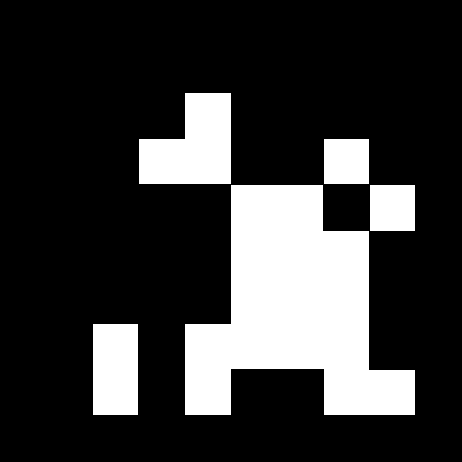
\includegraphics[width=0.8\linewidth]{markers/vector/apriltag_id0.pdf}
        \caption{AprilTag 36h11 (Вектор)}
    \end{minipage}
\end{figure}

\begin{figure}[H]
    \centering
    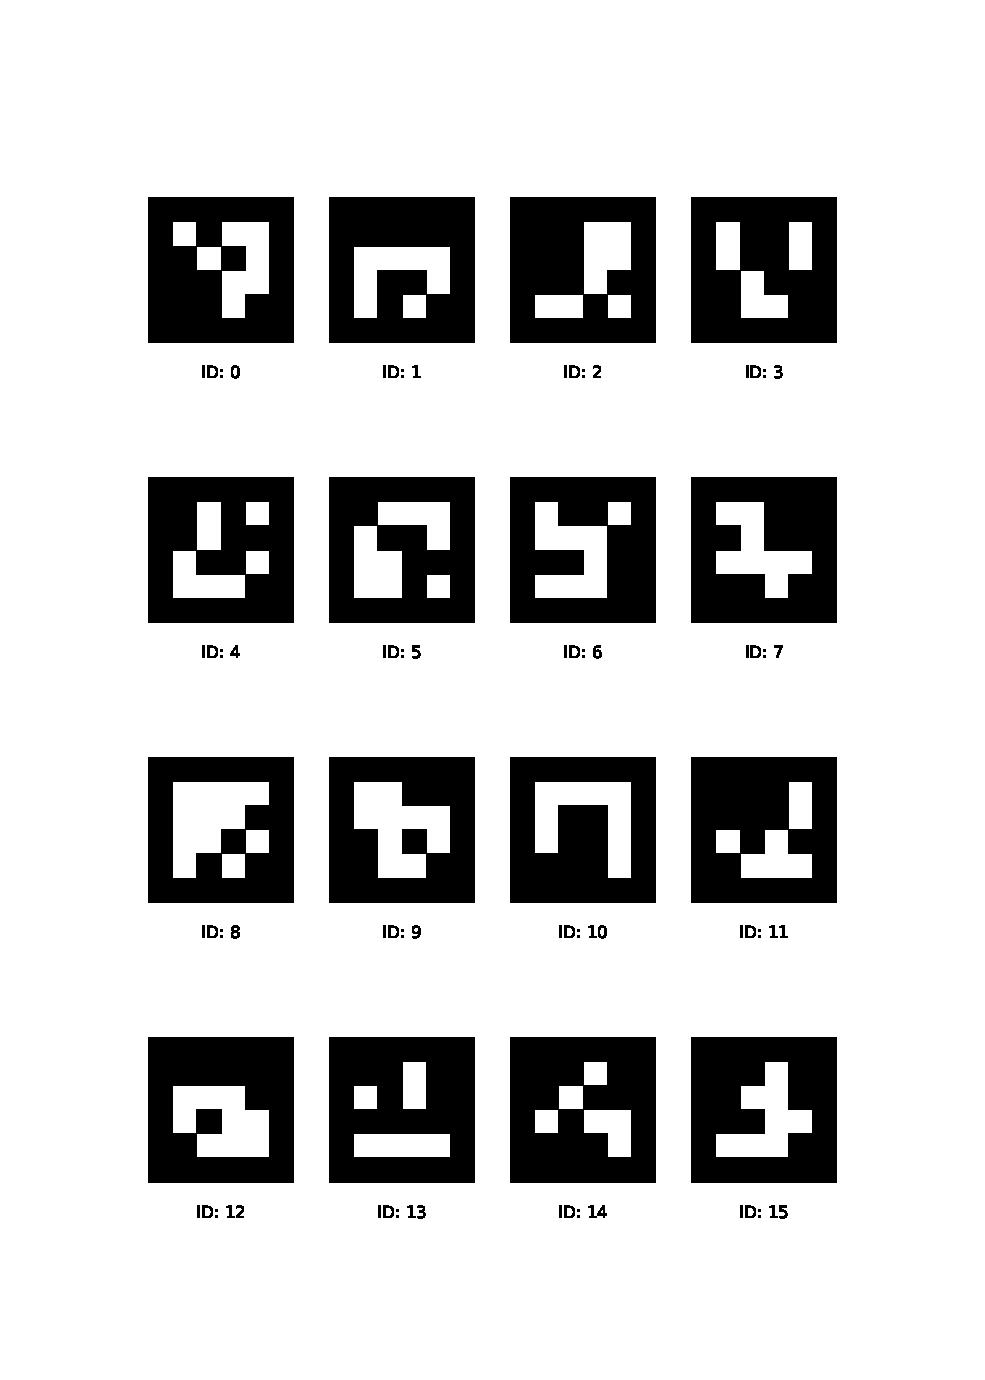
\includegraphics[width=0.9\linewidth]{markers/vector/aruco_grid_4x4.pdf}
    \caption{Карта маркеров 4x4 (ArUco, вектор)}
\end{figure}

\begin{warnbox}{Важно!}
При печати в настройках принтера выберите «Реальный размер» (Actual Size) или «Масштаб 100\%». Иначе размер маркера изменится, и навигация будет врать.
\end{warnbox}

\subsubsection{Требования к монтажу}
\begin{enumerate}
    \item \textbf{Жесткость:} Маркер должен быть идеально плоским. Изгиб бумаги даже на 5 мм приведет к ошибке определения угла (Yaw/Pitch/Roll) на 10-15 градусов. Наклейте маркер на картон, пластик или фанеру.
    \item \textbf{Quiet Zone:} Вокруг черной рамки маркера обязательно должно быть белое поле шириной не менее одного бита. Если наклеить черный маркер на черный пол, он не распознается.
    \item \textbf{Матовое покрытие:} Глянцевая бумага или скотч создают блики от ламп. В месте блика камера видит белое пятно вместо черного пикселя. Используйте матовую ламинацию или матовый скотч.
    \item \textbf{Освещение:} Избегайте размещения маркеров в глубокой тени или напротив ярких окон (контражур).
\end{enumerate}

\subsection{Форматы карт (JSON, XML, KML)}
Карта маркеров — это файл, описывающий положение каждого маркера. Наш инструмент \texttt{19\_map\_creation\_example3\_builder.py} поддерживает несколько форматов.

\begin{codefiletitle}[python]{Инструмент создания карт}{python/advanced_navigation/19_map_creation_example3_builder.py}
\end{codefiletitle}

\subsubsection{JSON (JavaScript Object Notation)}
Основной формат для роботов. Легко читается программами на Python/C++.
\begin{codefiletitle}[python]{Пример карты JSON}{python/advanced_navigation/map_json_example.json}
\end{codefiletitle}

\subsubsection{XML (eXtensible Markup Language)}
Более строгий формат, часто используется в промышленных системах.
\begin{codefiletitle}[xml]{Пример карты XML}{python/advanced_navigation/map_xml_example.xml}
\end{codefiletitle}

\subsubsection{KML (Keyhole Markup Language)}
Формат для отображения на географических картах (Google Earth, QGIS). Позволяет визуализировать схему расположения маркеров поверх спутниковых снимков. Это полезно для планирования полетов на улице.

\subsection{Визуализация и планирование}
Для больших полигонов рекомендуется сначала создать план в CAD-системе или нарисовать схему на миллиметровке, определить координаты установки маркеров, и только потом заносить их в файл карты.

\begin{taskbox}[Задание 3: Калибровка]
Проведите процедуру калибровки камеры Pioneer.
1. Сделайте 20 снимков шахматной доски.
2. Запустите скрипт калибровки.
3. Сравните изображение до и после устранения дисторсии (функция \texttt{cv2.undistort}). Прямые ли линии косяков дверей на краях кадра?
\end{taskbox}

\begin{taskbox}[Задание 4: Создание полигона]
Создайте карту для полета <<восьмеркой>>.
1. Нарисуйте траекторию на полу мелом.
2. Разместите 2 маркера в центрах петель восьмерки.
3. Измерьте их координаты рулеткой относительно точки старта.
4. Создайте JSON файл карты.
\end{taskbox}

\begin{questionbox}[Контрольные вопросы]
\begin{enumerate}
    \item Что такое дисторсия и почему она мешает навигации?
    \item Почему нельзя ламинировать маркеры глянцевой пленкой?
    \item Зачем нужно белое поле вокруг маркера?
    \item В чем преимущество формата KML перед JSON?
\end{enumerate}
\end{questionbox}
